%%%%%%%%%%%%%%%%%%%%%%%%%%%%%%%%%%%%%%%%%%%%%%%%%%%%%%%%%%%%%%%%%%%%%%%

\chapter{Experiment 1: Sensor Interfacing}

This chapter presents Arduino-based sensor interfacing experiments carried out during the internship. These experiments demonstrate the integration of environmental sensors, display modules, and actuators to develop real-time monitoring and automation systems.

%%%%%%%%%%%%%%%%%%%%%%%%%%%%%%%%%%%%%%%%%%%%%%%%%%%%%%%%%%%%%%%%%%%%%%%

\section{Digital Temperature Monitoring System}

%%%%%%%%%%%%%%%%%%%%%%%%%%%%%%%%%%%%%%%%%%%%%%%%%%%%%%%%%%%%%%%%%%%%%%%

\subsection{Problem Statement}

The main objective of this project is to design a smart temperature monitoring system using Arduino UNO and a DHT11 temperature sensor.

The system continuously measures room temperature and displays the live temperature value on an SSD1306 OLED display. According to the temperature value, the system automatically controls cooling and heating devices such as a fan and heater.

A push button is also provided to turn the complete system ON or OFF manually.

%%%%%%%%%%%%%%%%%%%%%%%%%%%%%%%%%%%%%%%%%%%%%%%%%%%%%%%%%%%%%%%%%%%%%%%

\subsection{Components Used \& Pin Connections}

\begin{table}[H]
\centering

\begin{minipage}[t]{0.55\textwidth}
\centering
\caption{Temperature Monitoring Components}
\label{tab:temp_components}

\begin{tabular}{|p{5cm}|c|}
\hline
\textbf{Component} & \textbf{Quantity} \\
\hline
Arduino UNO & 1 \\
DHT11 Temperature Sensor & 1 \\
SSD1306 OLED Display & 1 \\
Red LED & 1 \\
Green LED & 1 \\
DC Fan / Motor & 1 \\
Heater / Bulb & 1 \\
Push Button & 1 \\
Jumper Wires & Required \\
\hline
\end{tabular}

\end{minipage}
\hfill
\begin{minipage}[t]{0.40\textwidth}
\centering
\caption{Temperature Monitoring Pin Connections}
\label{tab:temp_pins}

\begin{tabular}{|l|c|}
\hline
\textbf{Device} & \textbf{Arduino Pin} \\
\hline
DHT11 Data Pin & D2 \\
Red LED & D3 \\
Green LED & D4 \\
Push Button & D7 \\
Heater & D8 \\
Fan & D9 \\
OLED SDA & A4 \\
OLED SCL & A5 \\
\hline
\end{tabular}

\end{minipage}

\end{table}

%%%%%%%%%%%%%%%%%%%%%%%%%%%%%%%%%%%%%%%%%%%%%%%%%%%%%%%%%%%%%%%%%%%%%%%
\clearpage
\subsection{Software Used}

\begin{itemize}
    \item Arduino IDE
    \item SimulIDE
\end{itemize}

%%%%%%%%%%%%%%%%%%%%%%%%%%%%%%%%%%%%%%%%%%%%%%%%%%%%%%%%%%%%%%%%%%%%%%%

\subsection{Circuit Diagram}

\begin{figure}[H]
\centering

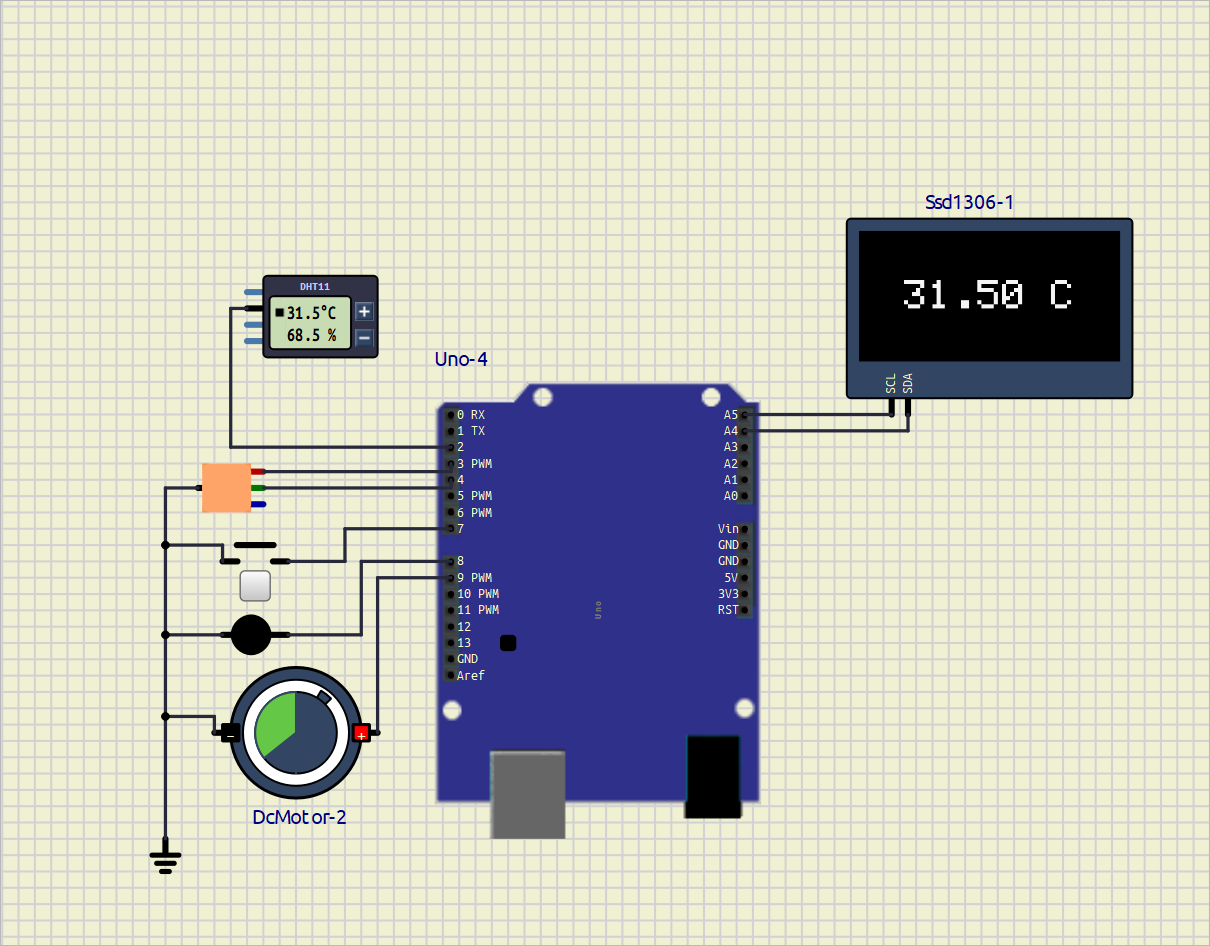
\includegraphics[width=0.80\textwidth]{Exp-1/smart_temp_controler/temp_sys_circuit.png}

\caption{Digital Temperature Monitoring System Circuit Diagram}
\label{fig:temp_monitor}

\end{figure}

%%%%%%%%%%%%%%%%%%%%%%%%%%%%%%%%%%%%%%%%%%%%%%%%%%%%%%%%%%%%%%%%%%%%%%%

\subsection{Source Code}

The complete Arduino source code for this experiment is available in the project repository.

\href{https://github.com/YOUR_USERNAME/YOUR_REPOSITORY/blob/main/Exp-1/smart_temp_controler/temp_sys.ino}
{\textbf{Click here to view the Arduino Source Code}}

%%%%%%%%%%%%%%%%%%%%%%%%%%%%%%%%%%%%%%%%%%%%%%%%%%%%%%%%%%%%%%%%%%%%%%%

%%%%%%%%%%%%%%%%%%%%%%%%%%%%%%%%%%%%%%%%%%%%%%%%%%%%%%%%%%%%%%%%%%%%%%%

\subsection{Working Principle}

\begin{enumerate}

\item The push button is used to turn the complete system ON or OFF.

\item When the system is ON, the DHT11 sensor continuously measures the room temperature.

\item The measured temperature value is displayed on the SSD1306 OLED display in real time.

\item Arduino UNO continuously compares the measured temperature with the predefined threshold value of 28$^\circ$C.

\item If the temperature becomes greater than or equal to 28$^\circ$C:

\begin{itemize}
    \item Red LED turns ON.
    \item Fan starts running automatically.
    \item Heater turns OFF.
\end{itemize}

\item If the temperature becomes lower than 28$^\circ$C:

\begin{itemize}
    \item Green LED turns ON.
    \item Heater turns ON automatically.
    \item Fan turns OFF.
\end{itemize}

\item The OLED display continuously updates the live temperature reading.

\item When the push button is pressed again:

\begin{itemize}
    \item The complete system turns OFF.
    \item OLED display becomes blank.
    \item LEDs turn OFF.
    \item Fan and heater stop working.
\end{itemize}

\end{enumerate}


%%%%%%%%%%%%%%%%%%%%%%%%%%%%%%%%%%%%%%%%%%%%%%%%%%%%%%%%%%%%%%%%%%%%%%%

\subsection{Conclusion}

The Digital Temperature Monitoring System using Arduino UNO and the DHT11 temperature sensor was successfully implemented and tested in SimulIDE.

The system continuously monitored room temperature and automatically controlled the fan and heater according to the measured temperature. The SSD1306 OLED display successfully showed the live temperature reading, while the push button provided convenient ON/OFF control of the complete system.

This project helped to understand the following:

\begin{itemize}

\item Arduino interfacing

\item Sensor interfacing

\item OLED display handling

\item Embedded system automation

\item Temperature-based control systems

\end{itemize}

%%%%%%%%%%%%%%%%%%%%%%%%%%%%%%%%%%%%%%%%%%%%%%%%%%%%%%%%%%%%%%%%%%%%%%%

\subsection{References}

\begin{enumerate}

\item Arduino UNO Documentation

\url{https://docs.arduino.cc/hardware/uno-rev3/}

\item DHT11 Sensor Documentation

\url{https://components101.com/sensors/dht11-temperature-sensor}

\item Adafruit SSD1306 Library

\url{https://github.com/adafruit/Adafruit_SSD1306}

\item Adafruit GFX Library

\url{https://github.com/adafruit/Adafruit-GFX-Library}

\item Arduino DHT Sensor Library

\url{https://docs.arduino.cc/libraries/dht-sensor-library/}

\item Arduino UNO Pinout

\url{https://deepbluembedded.com/arduino-uno-pinout/}

\end{enumerate}

%%%%%%%%%%%%%%%%%%%%%%%%%%%%%%%%%%%%%%%%%%%%%%%%%%%%%%%%%%%%%%%%%%%%%%%

\clearpage
Experiment 1 (Go Further 1):

\section{Temperature Monitoring \& Alert System}
%%%%%%%%%%%%%%%%%%%%%%%%%%%%%%%%%%%%%%%%%%%%%%%%%%%%%%%%%%%%%%%%%%%%%%%

\subsection{Problem Statement}

This project monitors temperature using a DHT11 sensor and activates a buzzer when the temperature exceeds the threshold value of 50$^\circ$C. The system is designed using Arduino UNO in SimulIDE.

%%%%%%%%%%%%%%%%%%%%%%%%%%%%%%%%%%%%%%%%%%%%%%%%%%%%%%%%%%%%%%%%%%%%%%%

\subsection{Components Used \& Pin Connections}

\begin{table}[H]
\centering

\begin{minipage}[t]{0.52\textwidth}
\centering
\caption{Emergency Alert System Components}
\label{tab:alert_components}

\begin{tabular}{|p{4cm}|c|}
\hline
\textbf{Component} & \textbf{Quantity} \\
\hline
Arduino UNO & 1 \\
DHT11 Temperature Sensor & 1 \\
Buzzer & 1 \\
Jumper Wires & Required \\
\hline
\end{tabular}

\end{minipage}
\hfill
\begin{minipage}[t]{0.42\textwidth}
\centering
\caption{Emergency Alert System Pin Connections}
\label{tab:alert_pins}

\begin{tabular}{|l|c|}
\hline
\textbf{Device} & \textbf{Arduino Pin} \\
\hline
DHT11 Data Pin & D1 \\
Buzzer & D8 \\
DHT11 VCC & 5V \\
DHT11 GND & GND \\
\hline
\end{tabular}

\end{minipage}

\end{table}

%%%%%%%%%%%%%%%%%%%%%%%%%%%%%%%%%%%%%%%%%%%%%%%%%%%%%%%%%%%%%%%%%%%%%%%

\subsection{Software Used}

\begin{itemize}
    \item Arduino IDE
    \item SimulIDE
\end{itemize}

%%%%%%%%%%%%%%%%%%%%%%%%%%%%%%%%%%%%%%%%%%%%%%%%%%%%%%%%%%%%%%%%%%%%%%%

\subsection{Circuit Diagram}

\begin{figure}[H]
\centering

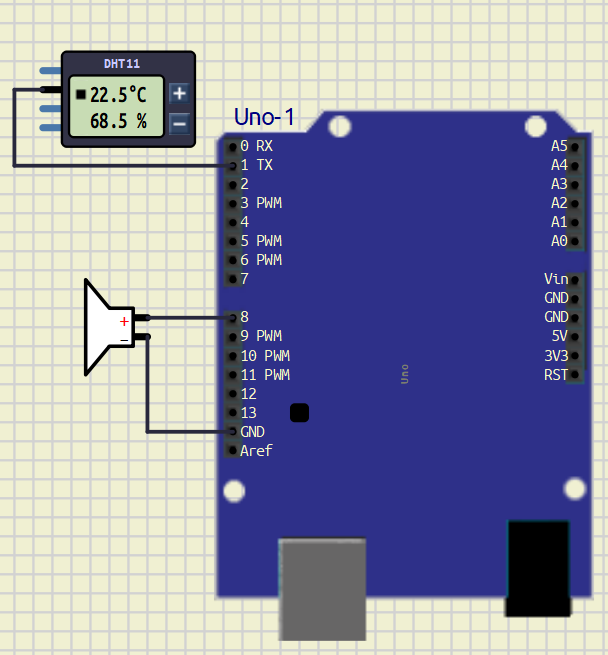
\includegraphics[width=0.37\textwidth]{Exp-1/temp_alert_sys/Circuit.png}

\caption{Temperature Monitoring-Emergency Alert System Circuit Diagram}
\label{fig:temp_alert}

\end{figure}

%%%%%%%%%%%%%%%%%%%%%%%%%%%%%%%%%%%%%%%%%%%%%%%%%%%%%%%%%%%%%%%%%%%%%%%

\subsection{Source Code}

The complete Arduino source code for this experiment is available in the project repository.

\href{https://github.com/YOUR_USERNAME/YOUR_REPOSITORY/blob/main/Exp-1/temp_alert_sys/temp_alert_sys.ino}
{\textbf{Click here to view the Arduino Source Code}}

%%%%%%%%%%%%%%%%%%%%%%%%%%%%%%%%%%%%%%%%%%%%%%%%%%%%%%%%%%%%%%%%%%%%%%%
%%%%%%%%%%%%%%%%%%%%%%%%%%%%%%%%%%%%%%%%%%%%%%%%%%%%%%%%%%%%%%%%%%%%%%%

\subsection{Working Principle}

\begin{enumerate}

\item The DHT11 temperature sensor continuously measures the surrounding temperature.

\item Arduino UNO continuously reads the temperature value from the DHT11 sensor.

\item The measured temperature is compared with the predefined threshold value of 50$^\circ$C.

\item If the temperature becomes greater than or equal to 50$^\circ$C:

\begin{itemize}
    \item The buzzer turns ON.
    \item A temperature alert is generated.
\end{itemize}

\item If the temperature remains below 50$^\circ$C:

\begin{itemize}
    \item The buzzer remains OFF.
\end{itemize}

\item The monitoring process repeats continuously with a delay of one second between consecutive readings.

\end{enumerate}

%%%%%%%%%%%%%%%%%%%%%%%%%%%%%%%%%%%%%%%%%%%%%%%%%%%%%%%%%%%%%%%%%%%%%%%

\subsection{Output}

\begin{itemize}

\item Buzzer remains OFF below 50$^\circ$C.

\item Buzzer turns ON at or above 50$^\circ$C.

\item System performs real-time temperature monitoring.

\end{itemize}

%%%%%%%%%%%%%%%%%%%%%%%%%%%%%%%%%%%%%%%%%%%%%%%%%%%%%%%%%%%%%%%%%%%%%%%

\subsection{Conclusion}

The Temperature Monitoring-Emergency Alert System using Arduino UNO and the DHT11 temperature sensor was successfully implemented and tested in SimulIDE.

The system continuously monitored the surrounding temperature and activated the buzzer whenever the measured temperature exceeded the predefined threshold value of 50$^\circ$C. This project demonstrated a simple and effective temperature-based emergency alert mechanism suitable for embedded monitoring applications.

%%%%%%%%%%%%%%%%%%%%%%%%%%%%%%%%%%%%%%%%%%%%%%%%%%%%%%%%%%%%%%%%%%%%%%%

\subsection{References}

\begin{enumerate}

\item Arduino Project Hub – Using DHT11 Sensor

\url{https://projecthub.arduino.cc/arcaegecengiz/using-dht11-12f621}

\item Arduino DHT Sensor Library

\url{https://docs.arduino.cc/libraries/dht-sensor-library/}

\item Arduino UNO Pinout

\url{https://deepbluembedded.com/arduino-uno-pinout/}

\end{enumerate}

%%%%%%%%%%%%%%%%%%%%%%%%%%%%%%%%%%%%%%%%%%%%%%%%%%%%%%%%%%%%%%%%%%%%%%%

\clearpage
Experiment 1 (Go Further 2):
\section{Weather Forecasting System}
%%%%%%%%%%%%%%%%%%%%%%%%%%%%%%%%%%%%%%%%%%%%%%%%%%%%%%%%%%%%%%%%%%%%%%%

\subsection{Problem Statement}

This project monitors the environmental temperature and humidity using a DHT-11 sensor and predicts weather conditions based on temperature readings.

The system uses an RGB LED to indicate different weather conditions:

\begin{itemize}
    \item Extreme Hot Weather
    \item Normal Weather
    \item Cold Weather
\end{itemize}

A DS1307 RTC module provides real-time clock information, while an SSD1306 OLED display continuously shows:

\begin{itemize}
    \item Current Time
    \item Temperature
    \item Humidity
    \item Weather Status
\end{itemize}

A push button is also provided as a master power control to turn the entire system ON and OFF.

%%%%%%%%%%%%%%%%%%%%%%%%%%%%%%%%%%%%%%%%%%%%%%%%%%%%%%%%%%%%%%%%%%%%%%%

\subsection{Components Used \& Pin Connections}

\begin{table}[H]
\centering

\begin{minipage}[t]{0.52\textwidth}
\centering
\caption{Weather Forecasting System Components}
\label{tab:weather_components}

\begin{tabular}{|p{4.2cm}|c|}
\hline
\textbf{Component} & \textbf{Quantity} \\
\hline
Arduino UNO & 1 \\
DHT11 Sensor & 1 \\
DS1307 RTC Module & 1 \\
SSD1306 OLED Display & 1 \\
RGB LED & 1 \\
Push Button & 1 \\
100$\Omega$ Resistors & 3 \\
Jumper Wires & Required \\
Breadboard & 1 \\
\hline
\end{tabular}

\end{minipage}
\hfill
\begin{minipage}[t]{0.43\textwidth}
\centering
\caption{Weather Forecasting Pin Connections}
\label{tab:weather_pins}

\begin{tabular}{|l|c|}
\hline
\textbf{Device} & \textbf{Arduino Pin} \\
\hline
DHT11 Data Pin & D7 \\
Red LED & D2 \\
Green LED & D3 \\
Blue LED & D5 \\
Power Button & D8 \\
OLED SDA & A4 \\
OLED SCL & A5 \\
RTC SDA & A4 \\
RTC SCL & A5 \\
\hline
\end{tabular}

\end{minipage}

\end{table}

%%%%%%%%%%%%%%%%%%%%%%%%%%%%%%%%%%%%%%%%%%%%%%%%%%%%%%%%%%%%%%%%%%%%%%%

\subsection{RGB LED Connections}

\begin{table}[H]
\centering
\caption{RGB LED Connections}
\label{tab:rgb_connections}

\begin{tabular}{|l|l|}
\hline
\textbf{RGB Pin} & \textbf{Connection} \\
\hline
Red Pin & D2 through 100$\Omega$ resistor \\
Green Pin & D3 through 100$\Omega$ resistor \\
Blue Pin & D5 through 100$\Omega$ resistor \\
Common Cathode & GND \\
\hline
\end{tabular}

\end{table}

%%%%%%%%%%%%%%%%%%%%%%%%%%%%%%%%%%%%%%%%%%%%%%%%%%%%%%%%%%%%%%%%%%%%%%%

\subsection{Software Used}

\begin{itemize}
    \item Arduino IDE
    \item SimulIDE
\end{itemize}

%%%%%%%%%%%%%%%%%%%%%%%%%%%%%%%%%%%%%%%%%%%%%%%%%%%%%%%%%%%%%%%%%%%%%%%

\subsection{Circuit Diagram}

\begin{figure}[H]
\centering


\includegraphics[width=0.70\textwidth]{Exp-1/weather_forcasting/circuit.png}

\caption{Weather Forecasting System Circuit Diagram}
\label{fig:weather_system}

\end{figure}

%%%%%%%%%%%%%%%%%%%%%%%%%%%%%%%%%%%%%%%%%%%%%%%%%%%%%%%%%%%%%%%%%%%%%%%

\subsection{Source Code}

The complete Arduino source code for this experiment is available in the project repository.

\href{https://github.com/YOUR_USERNAME/YOUR_REPOSITORY/blob/main/Exp-1/weather_forecast_system/weather_forecast_system.ino}
{\textbf{Click here to view the Arduino Source Code}}

%%%%%%%%%%%%%%%%%%%%%%%%%%%%%%%%%%%%%%%%%%%%%%%%%%%%%%%%%%%%%%%%%%%%%%%
%%%%%%%%%%%%%%%%%%%%%%%%%%%%%%%%%%%%%%%%%%%%%%%%%%%%%%%%%%%%%%%%%%%%%%%

\subsection{Working Principle}

\begin{enumerate}

\item The system starts with a blank OLED display.

\item Pressing the power button:
\begin{itemize}
    \item Turns the system ON.
    \item Displays \texttt{POWER ON} on the OLED display.
\end{itemize}

\item The DHT11 sensor continuously measures:
\begin{itemize}
    \item Temperature
    \item Humidity
\end{itemize}

\item The DS1307 RTC module continuously provides the real-time clock.

\item The OLED display continuously shows:
\begin{itemize}
    \item Current Time
    \item Temperature
    \item Humidity
    \item Weather Status
\end{itemize}

\item The RGB LED indicates the weather condition:
\begin{itemize}
    \item Red LED $\rightarrow$ Extreme Hot Weather
    \item Green LED $\rightarrow$ Normal Weather
    \item Blue LED $\rightarrow$ Cold Weather
\end{itemize}

\item Pressing the power button again:
\begin{itemize}
    \item Displays \texttt{POWER OFF}
    \item Turns OFF all LEDs
    \item OLED returns to a blank screen
\end{itemize}

\end{enumerate}

%%%%%%%%%%%%%%%%%%%%%%%%%%%%%%%%%%%%%%%%%%%%%%%%%%%%%%%%%%%%%%%%%%%%%%%

\subsection{Temperature Indicator Logic}

\begin{table}[H]
\centering
\caption{Temperature Indicator Logic}
\label{tab:weather_indicator}

\begin{tabular}{|c|c|c|}
\hline
\textbf{Temperature} & \textbf{LED Status} & \textbf{Weather Condition} \\
\hline
$>$ 35$^\circ$C & Red LED ON & Extreme Hot \\
20$^\circ$C -- 35$^\circ$C & Green LED ON & Normal \\
$<$ 20$^\circ$C & Blue LED ON & Cold \\
\hline
\end{tabular}

\end{table}

%%%%%%%%%%%%%%%%%%%%%%%%%%%%%%%%%%%%%%%%%%%%%%%%%%%%%%%%%%%%%%%%%%%%%%%

\subsection{Output}

\begin{figure}[H]
\centering

%---------------- First Row ----------------%

\begin{minipage}{0.47\textwidth}
\centering
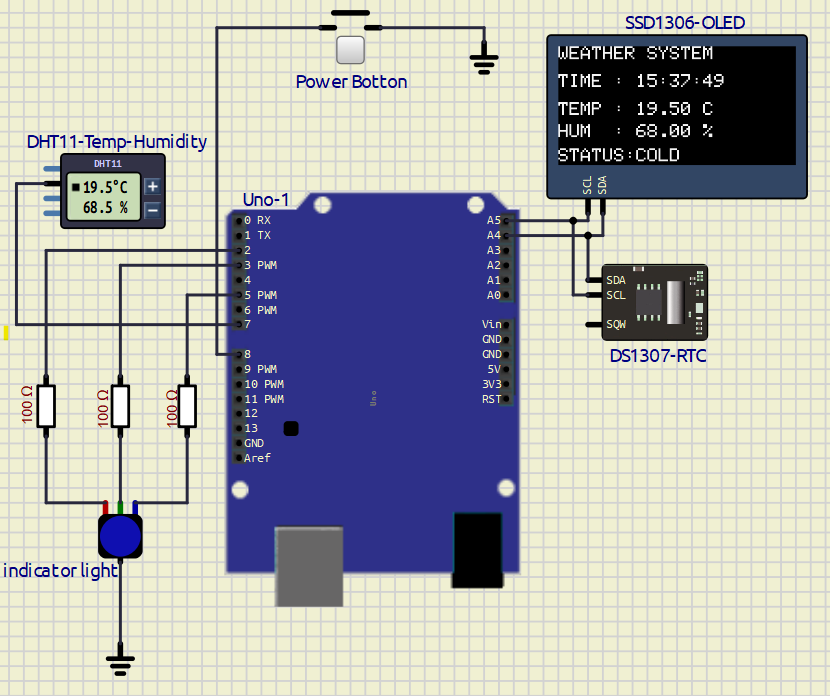
\includegraphics[width=\linewidth]{Exp-1/weather_forcasting/Cold.png}
\\
\small (a) Cold Weather
\end{minipage}
\hfill
\begin{minipage}{0.47\textwidth}
\centering
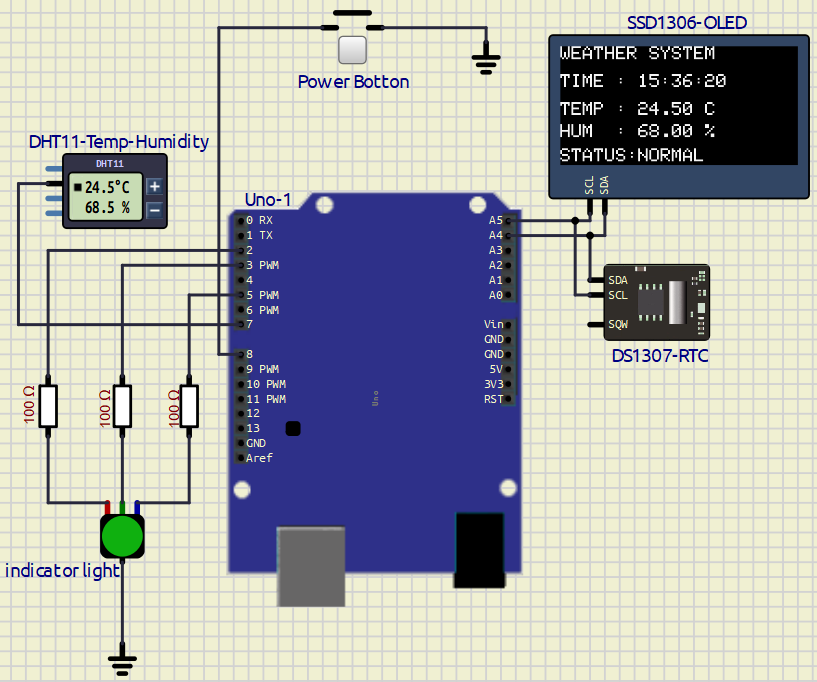
\includegraphics[width=\linewidth]{Exp-1/weather_forcasting/Normal.png}
\\
\small (b) Normal Weather
\end{minipage}

\vspace{0.5cm}

%---------------- Second Row ----------------%

\begin{minipage}{0.60\textwidth}
\centering
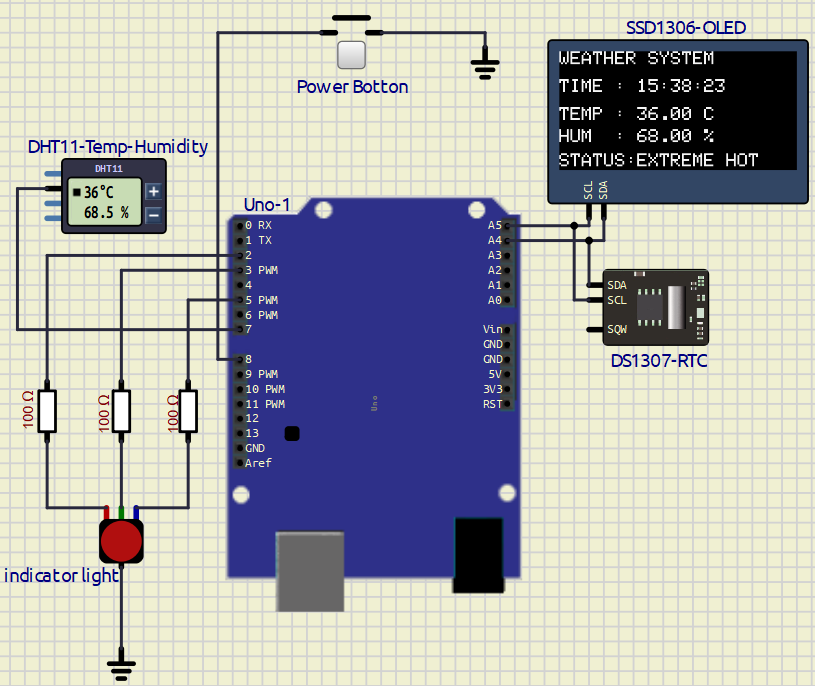
\includegraphics[width=\linewidth]{Exp-1/weather_forcasting/extreme_hot.png}
\\
\small (c) Extreme Hot Weather
\end{minipage}

\caption{Output of the Weather Forecasting System under different weather conditions}
\label{fig:weather_output}

\end{figure}


%%%%%%%%%%%%%%%%%%%%%%%%%%%%%%%%%%%%%%%%%%%%%%%%%%%%%%%%%%%%%%%%%%%%%%%

\subsection{Conclusion}

The Weather Forecasting System using Arduino UNO, DHT11 sensor, DS1307 RTC module, SSD1306 OLED display, RGB LED, and push-button control was successfully implemented and tested in SimulIDE.

The system correctly monitored weather conditions, displayed real-time environmental information, and visually indicated temperature conditions using RGB LEDs.
\clearpage
During this experiment, the following concepts were learned:

\begin{itemize}

\item Sensor interfacing

\item OLED interfacing

\item RTC interfacing

\item RGB LED control

\item Push-button logic

\item Embedded system design

\end{itemize}

%%%%%%%%%%%%%%%%%%%%%%%%%%%%%%%%%%%%%%%%%%%%%%%%%%%%%%%%%%%%%%%%%%%%%%%

\subsection{References}

\begin{enumerate}

\item Arduino UNO Documentation

\url{https://docs.arduino.cc/hardware/uno-rev3/}

\item DHT11 Sensor Documentation

\url{https://components101.com/sensors/dht11-temperature-sensor}

\item DS1307 RTC Datasheet

\url{https://datasheets.maximintegrated.com/en/ds/DS1307.pdf}

\item Adafruit SSD1306 Library

\url{https://github.com/adafruit/Adafruit_SSD1306}

\item Adafruit GFX Library

\url{https://github.com/adafruit/Adafruit-GFX-Library}

\item RTClib Documentation

\url{https://github.com/adafruit/RTClib}

\end{enumerate}

%%%%%%%%%%%%%%%%%%%%%%%%%%%%%%%%%%%%%%%%%%%%%%%%%%%%%%%%%%%%%%%%%%%%%%%

\clearpage

%%%%%%%%%%%%%%%%%%%%%%%%%%%%%%%%%%%%%%%%%%%%%%%%%%%%%%%%%%%%%%%%%%%%%%%
